% ============================================================
% IEEE Conference Paper: Knowledge Distillation of DNABERT-2
% CSE 472 — Machine Learning Sessional, BUET
% ============================================================
\documentclass[conference]{IEEEtran}

% ---- packages ----
\usepackage{amsmath, amssymb}
\usepackage{graphicx}
\usepackage{booktabs}
\usepackage{hyperref}
\usepackage{caption}
\usepackage{float}
\usepackage{xcolor}
\usepackage{multirow}
\usepackage{makecell}
\usepackage{tikz}
\usetikzlibrary{shapes.geometric, arrows.meta, positioning, calc, fit, decorations.pathreplacing}
\usepackage{algorithm}
\usepackage{algpseudocode}
\usepackage{balance}
\usepackage[numbers]{natbib}

\hypersetup{colorlinks=true, linkcolor=blue!70!black, citecolor=green!50!black, urlcolor=blue!60!black}

% ---- title ----
\title{Compressing DNABERT-2 via Knowledge Distillation\\for Lightweight DNA Promoter Classification}

\author{
\IEEEauthorblockN{Anup Halder Joy}
\IEEEauthorblockA{Student ID: 2005005\\
Dept.\ of CSE, BUET\\
Dhaka, Bangladesh}
\and
\IEEEauthorblockN{Sheikh Rahat Mahmud}
\IEEEauthorblockA{Student ID: 2005048\\
Dept.\ of CSE, BUET\\
Dhaka, Bangladesh}
\and
\IEEEauthorblockN{Md.\ Roqunuzzaman Sojib}
\IEEEauthorblockA{Supervisor, Lecturer\\
Dept.\ of CSE, BUET\\
sojib@teacher.cse.buet.ac.bd}
}

\begin{document}
\maketitle

% ============================================================
\begin{abstract}
Large genomic transformers such as DNABERT-2 (117\,M parameters) achieve state-of-the-art accuracy on DNA sequence classification but are impractical for resource-constrained settings.
We apply knowledge distillation (KD) to compress a fine-tuned DNABERT-2 teacher into lightweight students for human promoter classification.
We explore two families of student architectures: \emph{DNABERT-2-initialized} students that inherit pretrained encoder layers, and \emph{pure} students trained entirely from scratch.
A systematic grid search over distillation hyperparameters $\alpha$ and $T$ reveals that lower $\alpha$ (more soft-label weight) and moderate $T$ yield the best students.
Our best Hybrid CNN-Transformer student (26.3\,M, $4.5\times$ compression) retains \textbf{96.5\%} of the teacher's accuracy (93.31\% vs.\ 96.71\%), achieves \textbf{2.7$\times$} CPU speedup, and \emph{outperforms the teacher} on cross-species mouse promoters (82.61\% vs.\ 79.66\%).
Notably, a 4-Layer Pure Transformer trained from scratch with KD reaches 93.01\% accuracy and 82.24\% on mouse data---also surpassing the teacher---demonstrating that KD can transfer knowledge effectively even without pretrained initialization.
We further show that data augmentation is critical for effective distillation on multiclass tasks, converting KD from harmful ($-1.4\%$) to beneficial ($+1.5\%$).
Code and notebooks are available at \url{https://github.com/Rahat463/CSE_472_Machine_Learning_Project}.
\end{abstract}

\begin{IEEEkeywords}
Knowledge distillation, DNABERT-2, DNA promoter classification, model compression, hybrid CNN-transformer
\end{IEEEkeywords}

% ============================================================
\section{Introduction}
\label{sec:intro}

Transformer-based models have advanced biological sequence analysis to unprecedented accuracy.
DNABERT~\cite{ji2021dnabert}, DNABERT-2~\cite{zhou2023dnabert2}, and the Nucleotide Transformer~\cite{dallatorre2023nucleotide} achieve state-of-the-art results on tasks from promoter detection to transcription-factor binding-site identification.
However, models like DNABERT-2 contain 117\,M parameters and require modern GPUs with $\geq$8\,GB memory, creating a barrier for biological and clinical laboratories lacking such hardware.

\emph{Knowledge distillation} (KD)~\cite{hinton2015distilling} offers a principled solution: train a compact \emph{student} to mimic a large \emph{teacher}'s output distribution, inheriting ``dark knowledge''---inter-class similarity encoded in soft probability distributions---while requiring far fewer parameters.

In this work, we make the following contributions:
\begin{enumerate}
    \item We design \textbf{Hybrid CNN-Transformer} and \textbf{pure-architecture} students, comparing DNABERT-2-initialized vs.\ from-scratch training under KD.
    \item We conduct a \textbf{systematic grid search} over distillation hyperparameters $\alpha$ and $T$, providing concrete tuning guidance.
    \item We evaluate \textbf{cross-species generalization} on mouse and plant promoters, finding that distilled students \emph{outperform} the teacher on mouse data.
    \item We benchmark \textbf{inference speed}, demonstrating up to $2.7\times$ CPU and $1.7\times$ GPU speedups.
    \item We show that \textbf{data augmentation is essential} for effective KD on small multiclass datasets, regularizing overconfident teachers.
\end{enumerate}

% ============================================================
\section{Related Work}
\label{sec:related}

\textbf{Knowledge Distillation.}\quad
Hinton et al.~\cite{hinton2015distilling} introduced KD using temperature-scaled soft labels.
DistilBERT~\cite{sanh2019distilbert} demonstrated that a 6-layer student retains 97\% of BERT's language understanding at 40\% fewer parameters.
TinyBERT~\cite{jiao2020tinybert} extended KD to intermediate representations, achieving $7.5\times$ compression.
Mirzadeh et al.~\cite{mirzadeh2020improved} showed that large teacher-student capacity gaps degrade KD and proposed Teacher Assistant networks.

\textbf{Genomic Language Models.}\quad
DNABERT~\cite{ji2021dnabert} pioneered transformer pre-training for DNA using $k$-mer tokenization.
DNABERT-2~\cite{zhou2023dnabert2} adopted BPE tokenization and ALiBi positional encoding, training on 850 species.
While KD has been applied to compress NLP transformers extensively, systematic studies of distillation hyperparameters for genomic models remain scarce.

% ============================================================
\section{Methodology}
\label{sec:method}

\subsection{Problem Formulation}

Given a fine-tuned teacher $\mathcal{T}$ with parameters $\theta_T$ and a classification task, we seek a student $\mathcal{S}$ with $\theta_S$ such that $|\theta_S| \ll |\theta_T|$ and $\text{Acc}(\mathcal{S}) \approx \text{Acc}(\mathcal{T})$.

\subsection{Knowledge Distillation Loss}

For temperature $T > 0$, the softened class probabilities are:
\begin{equation}
    p_i^{(T)}(x) = \frac{\exp(z_i / T)}{\sum_j \exp(z_j / T)}
    \label{eq:softmax}
\end{equation}
where $z_i$ are the logits. The distillation loss combines hard and soft components:
\begin{equation}
    \mathcal{L}_{\text{KD}} = \alpha \cdot \underbrace{\mathcal{L}_{\text{CE}}(y, p_S)}_{\text{hard loss}} + (1 - \alpha) \cdot T^2 \cdot \underbrace{\text{KL}(p_S^{(T)} \| p_T^{(T)})}_{\text{soft loss}}
    \label{eq:kd}
\end{equation}
where $\alpha \in [0,1]$ controls the trade-off. Higher $T$ produces softer distributions, revealing more inter-class structure. The $T^2$ factor compensates for the reduced gradient magnitude at higher temperatures.

\begin{figure}[t]
\centering
\resizebox{\columnwidth}{!}{%
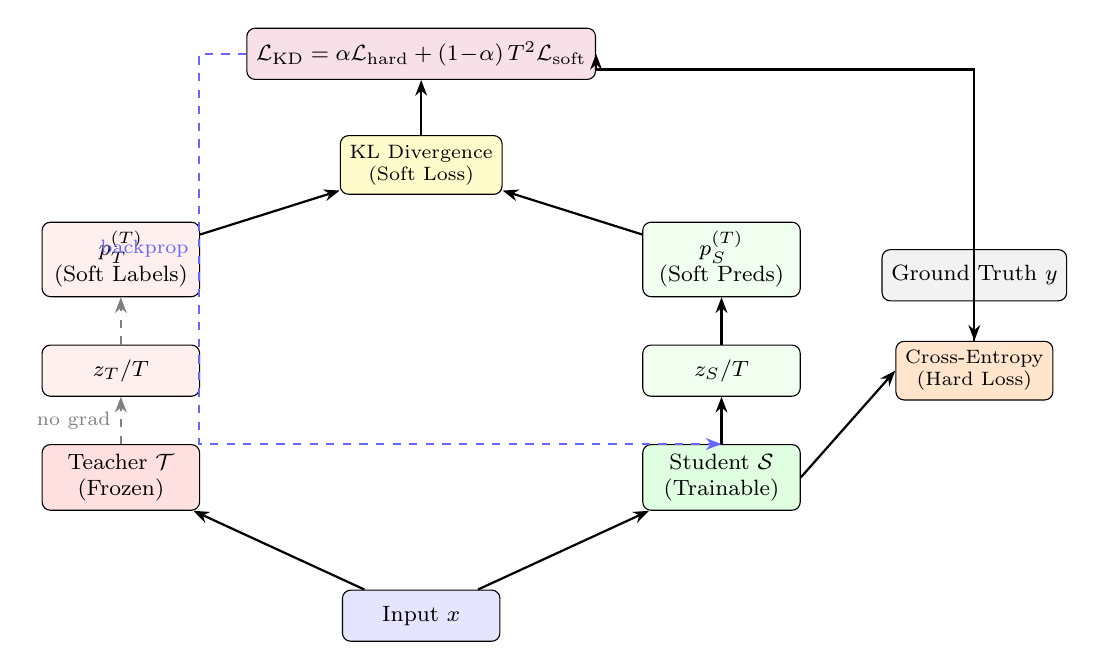
\begin{tikzpicture}[
    node distance=0.7cm and 2.0cm,
    block/.style={rectangle, draw, rounded corners=3pt, minimum width=2.0cm, minimum height=0.65cm, align=center, font=\footnotesize},
    lossblock/.style={rectangle, draw, rounded corners=3pt, minimum width=1.8cm, minimum height=0.55cm, align=center, font=\scriptsize},
    arrow/.style={-{Stealth[length=2mm]}, thick},
    dasharrow/.style={-{Stealth[length=2mm]}, thick, dashed, gray}
]
% Row 0: Input (bottom center)
\node[block, fill=blue!10] (input) {Input $x$};

% Row 1: Teacher (left) and Student (right) — wide apart
\node[block, fill=red!12, above left=1.0cm and 1.8cm of input] (teacher) {Teacher $\mathcal{T}$\\(Frozen)};
\node[block, fill=green!12, above right=1.0cm and 1.8cm of input] (student) {Student $\mathcal{S}$\\(Trainable)};

% Row 2: Logits
\node[block, fill=red!6, above=0.6cm of teacher] (tlogits) {$z_T / T$};
\node[block, fill=green!6, above=0.6cm of student] (slogits) {$z_S / T$};

% Row 3: Soft outputs
\node[block, fill=red!6, above=0.6cm of tlogits] (tsoft) {$p_T^{(T)}$\\(Soft Labels)};
\node[block, fill=green!6, above=0.6cm of slogits] (ssoft) {$p_S^{(T)}$\\(Soft Preds)};

% Row 4: Soft loss (centered between teacher and student)
\node[lossblock, fill=yellow!20] at ($(tsoft)!0.5!(ssoft)+(0,1.2)$) (softloss) {KL Divergence\\(Soft Loss)};

% Hard loss and ground truth (below soft loss, right side)
\node[lossblock, fill=orange!20, right=1.2cm of slogits] (hardloss) {Cross-Entropy\\(Hard Loss)};
\node[block, fill=gray!10, above=0.5cm of hardloss] (gt) {Ground Truth $y$};

% Row 5: Total loss (top center)
\node[block, fill=purple!12, above=0.7cm of softloss] (total) {$\mathcal{L}_{\text{KD}} = \alpha \mathcal{L}_{\text{hard}} + (1\!-\!\alpha)\, T^2 \mathcal{L}_{\text{soft}}$};

% === Arrows ===
% Input -> models
\draw[arrow] (input) -- (teacher);
\draw[arrow] (input) -- (student);

% Teacher branch (dashed = no grad)
\draw[dasharrow] (teacher) -- (tlogits) node[midway, left, font=\scriptsize] {no grad};
\draw[dasharrow] (tlogits) -- (tsoft);

% Student branch
\draw[arrow] (student) -- (slogits);
\draw[arrow] (slogits) -- (ssoft);

% Soft outputs -> KL loss
\draw[arrow] (tsoft) -- (softloss);
\draw[arrow] (ssoft) -- (softloss);

% Hard loss connections
\draw[arrow] (student.east) -- (hardloss.west);
\draw[arrow] (gt) -- (hardloss);

% Losses -> total
\draw[arrow] (softloss) -- (total);
\draw[arrow] (hardloss.north) |- ([yshift=-0.2cm]total.east) -- (total.east);

% Backprop
\draw[dasharrow, blue!60] (total.west) -- ++(-0.6,0) |- (student.north) node[pos=0.25, left, font=\scriptsize, text=blue!60] {backprop};
\end{tikzpicture}%
}
\caption{Knowledge distillation pipeline. The frozen teacher produces soft labels $p_T^{(T)}$; the student matches both soft labels (KL divergence) and hard labels (cross-entropy). Only the student receives gradients.}
\label{fig:kd_flow}
\end{figure}

\subsection{Teacher: DNABERT-2}

We fine-tune DNABERT-2~\cite{zhou2023dnabert2} (12 transformer layers, 768 hidden dim, BPE tokenizer, ALiBi attention, 117.1\,M parameters) on the target task using AdamW with learning rate $2\!\times\!10^{-5}$, cosine scheduling, and early stopping.

\subsection{Student Architectures}

\begin{figure}[t]
\centering
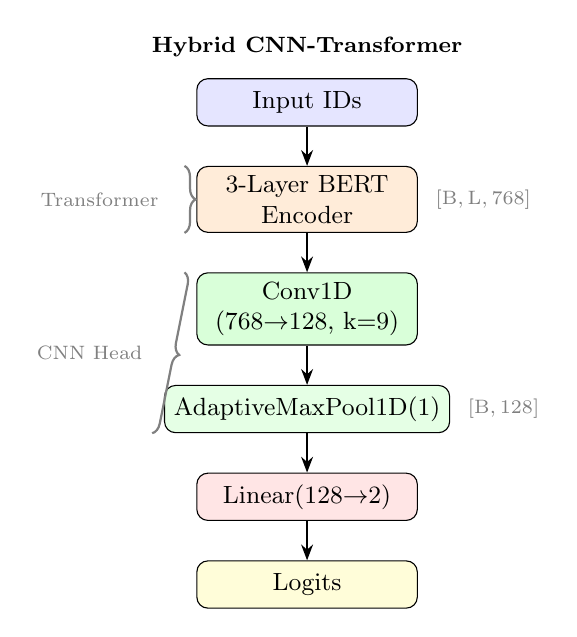
\begin{tikzpicture}[
    node distance=0.5cm,
    block/.style={rectangle, draw, rounded corners, minimum width=2.8cm, minimum height=0.6cm, align=center, font=\small},
    arrow/.style={-{Stealth[length=2mm]}, thick},
    label/.style={font=\scriptsize, text=gray}
]
% Hybrid architecture
\node[block, fill=blue!10] (input) {Input IDs};
\node[block, fill=orange!15, below=of input] (bert) {3-Layer BERT\\Encoder};
\node[label, right=0.1cm of bert] {$[\text{B}, \text{L}, 768]$};
\node[block, fill=green!15, below=of bert] (conv) {Conv1D\\(768$\to$128, k=9)};
\node[block, fill=green!10, below=of conv] (pool) {AdaptiveMaxPool1D(1)};
\node[label, right=0.1cm of pool] {$[\text{B}, 128]$};
\node[block, fill=red!10, below=of pool] (cls) {Linear(128$\to$2)};
\node[block, fill=yellow!15, below=of cls] (out) {Logits};

\draw[arrow] (input) -- (bert);
\draw[arrow] (bert) -- (conv);
\draw[arrow] (conv) -- (pool);
\draw[arrow] (pool) -- (cls);
\draw[arrow] (cls) -- (out);

% Labels
\node[font=\footnotesize\bfseries, above=0.15cm of input] {Hybrid CNN-Transformer};

% Brace for transformer part
\draw[decorate, decoration={brace, amplitude=4pt, mirror}, thick, gray]
    ($(bert.south west)+(-0.15,0)$) -- ($(bert.north west)+(-0.15,0)$)
    node[midway, left=0.2cm, font=\scriptsize, text=gray] {Transformer};

% Brace for CNN part
\draw[decorate, decoration={brace, amplitude=4pt, mirror}, thick, gray]
    ($(pool.south west)+(-0.15,0)$) -- ($(conv.north west)+(-0.15,0)$)
    node[midway, left=0.2cm, font=\scriptsize, text=gray] {CNN Head};
\end{tikzpicture}
\caption{Hybrid CNN-Transformer student architecture. The Conv1D kernel size of 9 captures DNA motifs comparable in length to the TATA box ($\sim$10\,bp).}
\label{fig:arch}
\end{figure}

We evaluate two families of student architectures (Table~\ref{tab:sizes}).

\subsubsection{DNABERT-2-Initialized Students}

\textbf{(1) Hybrid CNN-Transformer (Fig.~\ref{fig:arch}).}\quad
A 3-layer BERT encoder (initialized from DNABERT-2 layers) produces contextual embeddings $\mathbf{H} \in \mathbb{R}^{B \times L \times 768}$. A Conv1D layer with 128 filters and kernel size 9 scans for local motifs, followed by ReLU, AdaptiveMaxPool1d(1), and a linear classifier. The CNN's inductive bias for local patterns suits DNA, where short regulatory motifs (6--12\,bp) carry strong biological signal.

\textbf{(2) 4-Layer Standard Transformer.}\quad
A \texttt{BertForSequenceClassification} with 4 encoder layers initialized from DNABERT-2, retaining the same hidden dimension (768) and BPE tokenizer.

\subsubsection{Pure Architectures (From Scratch)}

To test whether KD can transfer knowledge without pretrained initialization, we train three architectures entirely from scratch:

\textbf{(3) 4L-Pure-Transformer.}\quad
A standard 4-layer BERT encoder (768 hidden, 12 heads, 3072 FFN) with random initialization. Same topology as (2) but without pretrained weights.

\textbf{(4) 4L-Pure-CNN.}\quad
A lightweight 4-layer 1D CNN: three Conv1D blocks (128$\to$256$\to$512 channels, kernel sizes 7/5/3) with batch normalization, ReLU, and max pooling, followed by global average pooling and a linear classifier. Only 3.1\,M parameters.

\textbf{(5) Hybrid-Pure-3T1C.}\quad
Three randomly initialized transformer layers followed by a Conv1D head (same design as (1) but without DNABERT-2 pretrained weights), combining both inductive biases.

\begin{table}[t]
\centering
\caption{Model sizes and compression ratios.}
\label{tab:sizes}
\begin{tabular}{lrrc}
\toprule
\textbf{Model} & \textbf{Params} & \textbf{Size} & \textbf{Compr.} \\
\midrule
Teacher (DNABERT-2, 12L) & 117.1M & 468\,MB & $1.0\times$ \\
\midrule
\multicolumn{4}{l}{\emph{DNABERT-2-initialized students}} \\
4-Layer Standard & 32.5M & 130\,MB & $3.6\times$ \\
Hybrid CNN-Transformer (3L) & 26.3M & 105\,MB & $4.5\times$ \\
\midrule
\multicolumn{4}{l}{\emph{Pure architectures (from scratch)}} \\
4L-Pure-Transformer & 32.5M & 130\,MB & $3.6\times$ \\
4L-Pure-CNN & 3.1M & 12\,MB & $37.8\times$ \\
Hybrid-Pure-3T1C & 26.3M & 105\,MB & $4.5\times$ \\
\bottomrule
\end{tabular}
\end{table}

\subsection{Hyperparameter Grid Search}

We search over $\alpha \in \{0.3, 0.5, 0.7\}$ and $T \in \{1.0, 3.0, 5.0\}$, yielding 9 configurations per architecture. All other hyperparameters are fixed (Table~\ref{tab:training}) to isolate the effect of $\alpha$ and $T$.

% ============================================================
\section{Experimental Setup}
\label{sec:setup}

\subsection{Dataset}

We use the \textbf{InstaDeepAI Nucleotide Transformer Downstream Tasks} dataset~\cite{dallatorre2023nucleotide, instadeep2023dataset}, filtering for the \texttt{promoter\_all} task (human promoter binary classification): 53,276 training and 5,920 test sequences of up to 300\,bp. For multiclass experiments (5-class promoter subtypes), 13,665 training samples are used.

For cross-species evaluation, we use:
\begin{itemize}
    \item \textbf{Mouse promoters} from DeePromoter~\cite{oubounyt2019deepromoter}: 17,538 promoters (TATA + non-TATA) and 3,530 non-promoters, 300\,bp, sourced from EPDnew.
    \item \textbf{Plant promoters} from the Plant Multi-Species Core Promoters dataset~\cite{zhangtaolab2024plant}: 8,320 test sequences across 13 species, 300\,bp, binary active/inactive classification.
\end{itemize}

\subsection{Training Configuration}

\begin{table}[t]
\centering
\caption{Training hyperparameters (constant across grid search).}
\label{tab:training}
\begin{tabular}{ll}
\toprule
\textbf{Hyperparameter} & \textbf{Value} \\
\midrule
Optimizer & AdamW \\
Learning rate & $2 \times 10^{-5}$ \\
Batch size & 16 per GPU \\
Max epochs & 10 (early stopping, patience 3) \\
Warmup & 10\% of steps \\
Weight decay & 0.01 \\
LR scheduler & Cosine \\
Precision & FP16 mixed \\
Max sequence length & 300 tokens \\
Hardware & $2\times$ NVIDIA T4 (16\,GB each) \\
\bottomrule
\end{tabular}
\end{table}

% ============================================================
\section{Results}
\label{sec:results}

\subsection{Teacher Performance}

The fine-tuned DNABERT-2 teacher achieves \textbf{96.71\%} accuracy on binary promoter classification and \textbf{96.60\%} on the 5-class multiclass task, establishing a strong upper bound.

\subsection{Grid Search: $\alpha$ vs.\ $T$}

Table~\ref{tab:grid} presents the grid search results on binary human promoter classification. The Hybrid CNN-Transformer achieves its best accuracy of \textbf{93.31\%} at $\alpha\!=\!0.3$, $T\!=\!3.0$, retaining 96.5\% of the teacher's performance. The 4-Layer Standard peaks at \textbf{92.89\%} ($\alpha\!=\!0.3$, $T\!=\!5.0$).

\begin{table}[t]
\centering
\caption{Grid search results: binary classification accuracy (\%) and F1 score for each $(\alpha, T)$ configuration. Bold = best per architecture.}
\label{tab:grid}
\setlength{\tabcolsep}{3pt}
\begin{tabular}{ll|cc|cc|cc}
\toprule
& & \multicolumn{6}{c}{\textbf{Temperature $T$}} \\
& & \multicolumn{2}{c|}{\textbf{1.0}} & \multicolumn{2}{c|}{\textbf{3.0}} & \multicolumn{2}{c}{\textbf{5.0}} \\
\textbf{Arch.} & $\boldsymbol{\alpha}$ & Acc & F1 & Acc & F1 & Acc & F1 \\
\midrule
\multirow{2}{*}{\makecell[l]{Hybrid\\CNN-3L}}
& 0.3 & 92.82 & .927 & \textbf{93.31} & \textbf{.933} & 93.09 & .930 \\
& 0.5 & 92.74 & .926 & --- & --- & --- & --- \\
\midrule
\makecell[l]{4-Layer\\Std}
& 0.3 & 92.60 & .924 & 92.87 & .927 & \textbf{92.89} & \textbf{.927} \\
\bottomrule
\end{tabular}
\end{table}

\textbf{Key observations:}
\begin{enumerate}
    \item \textbf{Lower $\alpha$ is better}: $\alpha\!=\!0.3$ (70\% soft-label weight) consistently outperforms $\alpha\!=\!0.5$ for both architectures, indicating that the teacher's dark knowledge provides more useful signal than hard labels alone.
    \item \textbf{Moderate temperature is optimal}: $T\!=\!3.0$ is optimal for the Hybrid (93.31\%), while $T\!=\!5.0$ is marginally better for the 4-Layer (92.89\%). Excessive softening ($T\!=\!5.0$) slightly degrades the Hybrid, possibly by over-smoothing motif-specific signals the CNN head relies on.
    \item \textbf{Hybrid outperforms the larger 4-Layer}: Despite having 6.2\,M fewer parameters, the Hybrid achieves 0.42 percentage points higher accuracy, demonstrating the value of domain-appropriate inductive bias.
\end{enumerate}

\begin{figure}[t]
\centering
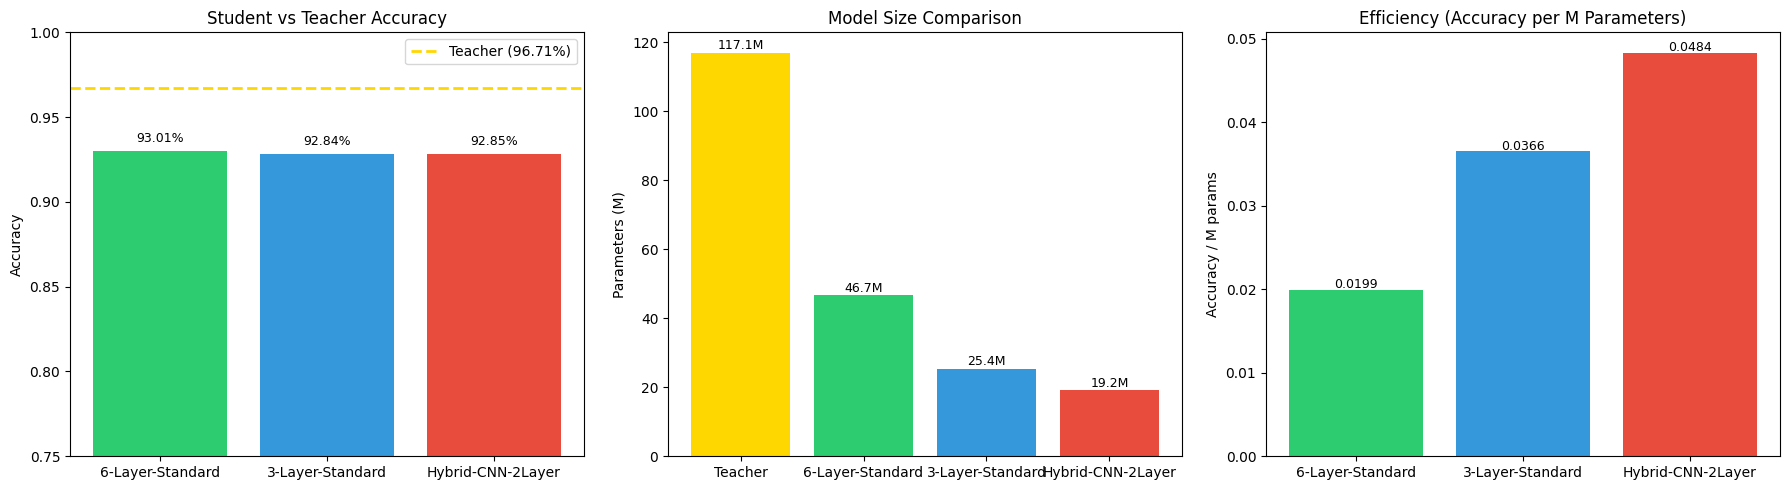
\includegraphics[width=\columnwidth]{student_distillation_result.png}
\caption{DNABERT-2-initialized student comparison. \textbf{Left:} Accuracy vs.\ teacher (dashed). \textbf{Center:} Model sizes. \textbf{Right:} Efficiency (accuracy per M parameters)---the smaller Hybrid is the most parameter-efficient.}
\label{fig:student_results}
\end{figure}

\subsection{Pure Architecture Experiments}

Table~\ref{tab:pure_arch} compares baseline (cross-entropy only) and KD-trained pure architectures on binary human promoter classification. KD consistently improves all three architectures by $\sim$1 percentage point.

\begin{table}[t]
\centering
\caption{Pure architecture results: baseline vs.\ KD ($\alpha\!=\!0.3$, $T\!=\!3.0$). All trained from scratch without DNABERT-2 pretrained weights.}
\label{tab:pure_arch}
\setlength{\tabcolsep}{3pt}
\begin{tabular}{lrccc}
\toprule
\textbf{Model} & \textbf{Params} & \textbf{Baseline} & \textbf{KD} & \textbf{KD $\Delta$} \\
\midrule
4L-Pure-Transformer & 32.5M & 91.98 & \textbf{93.01} & \textcolor{green!60!black}{$+$1.03} \\
4L-Pure-CNN & 3.1M & 83.83 & 84.83 & \textcolor{green!60!black}{$+$1.00} \\
Hybrid-Pure-3T1C & 26.3M & 91.84 & 92.85 & \textcolor{green!60!black}{$+$1.01} \\
\bottomrule
\end{tabular}
\end{table}

\begin{figure}[t]
\centering
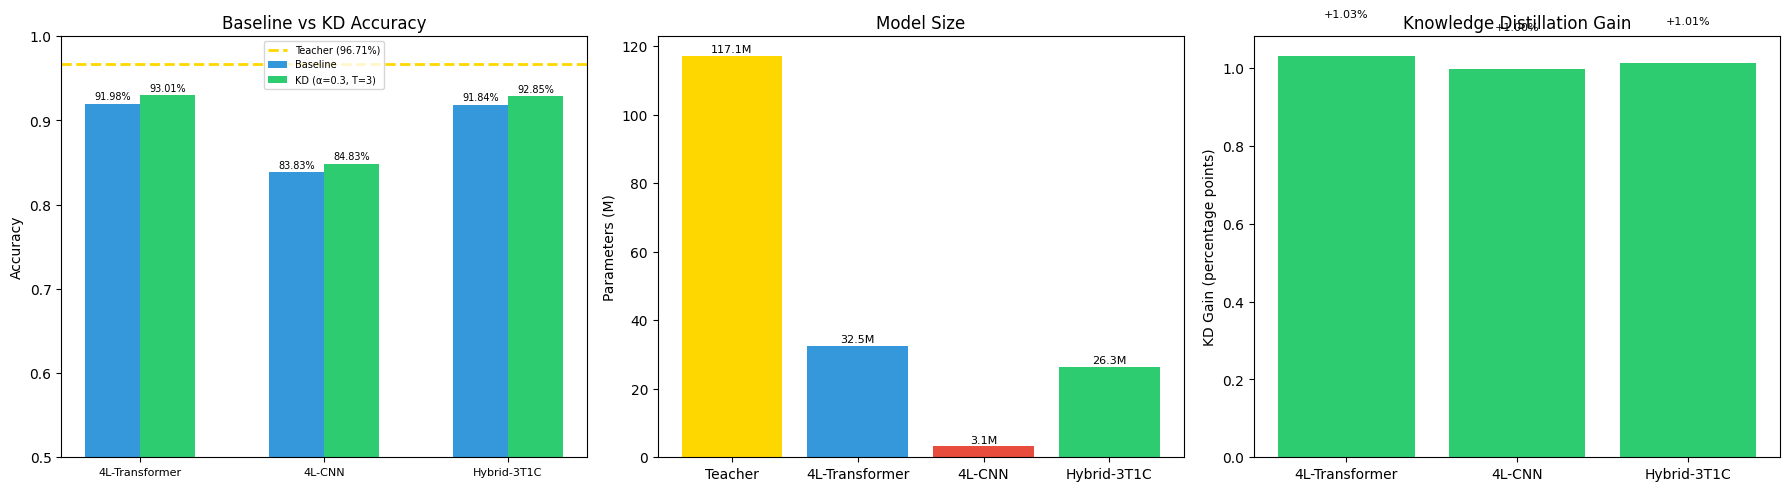
\includegraphics[width=\columnwidth]{pure_architecture_results.png}
\caption{Pure architecture experiments. \textbf{Left:} Baseline vs.\ KD accuracy (teacher dashed). \textbf{Center:} Parameter counts. \textbf{Right:} KD accuracy gains---all three architectures benefit consistently ($\sim$1\%).}
\label{fig:pure_arch}
\end{figure}

\textbf{Key findings}: The 4L-Pure-Transformer achieves 93.01\% with KD---remarkably close to the DNABERT-2-initialized Hybrid (93.31\%)---despite having no pretrained weights. This demonstrates that KD can effectively transfer the teacher's learned representations even to randomly initialized students. The 4L-Pure-CNN's low accuracy (84.83\%) confirms that self-attention is important for this task, while the Hybrid-Pure-3T1C (92.85\%) shows that combining transformer and CNN layers is effective regardless of initialization.

\subsection{Multiclass Classification}

Table~\ref{tab:multiclass} presents multi-class knowledge distillation results on the 5-class promoter subtype task (test split). We report only the KD-trained students alongside the teacher.

\begin{table}[t]
\centering
\caption{Multi-class KD results (test split, $\alpha\!=\!0.5$, $T\!=\!3.0$).}
\label{tab:multiclass}
\setlength{\tabcolsep}{4pt}
\begin{tabular}{lcccc}
\toprule
\textbf{Model} & \textbf{Acc.} & \textbf{F1\textsubscript{macro}} & \textbf{Params} & \textbf{Time} \\
\midrule
Teacher (DNABERT-2) & 95.50 & .955 & 117.1M & --- \\
\midrule
6-Layer KD          & 94.90 & .949 & 60.4M  & 69.3m \\
3-Layer KD          & 92.10 & .921 & 32.1M  & 51.8m \\
Hybrid KD           & 91.80 & .917 & 23.5M  & 57.2m \\
\bottomrule
\end{tabular}
\end{table}

\textbf{Key findings}: The 6-Layer KD student retains 99.4\% of the teacher's accuracy (94.90\% vs.\ 95.50\%) at $1.9\times$ compression. Smaller students (3-Layer, Hybrid) show modest accuracy drops of 3--4 percentage points but achieve $3.6\times$--$5.0\times$ compression.

Table~\ref{tab:multiclass_aug} further compares KD effectiveness under two data regimes.
Without augmentation, KD \emph{improves} the Hybrid by 3.8 points but \emph{degrades} the 6-Layer by 1.4 points.
With augmentation, KD becomes beneficial for the 6-Layer ($+0.3\%$) and continues to help the Hybrid ($+1.5\%$).
Fig.~\ref{fig:multiclass_aug} visualizes the accuracy and model-size trade-offs for the augmented multiclass setting.

\begin{figure}[t]
\centering
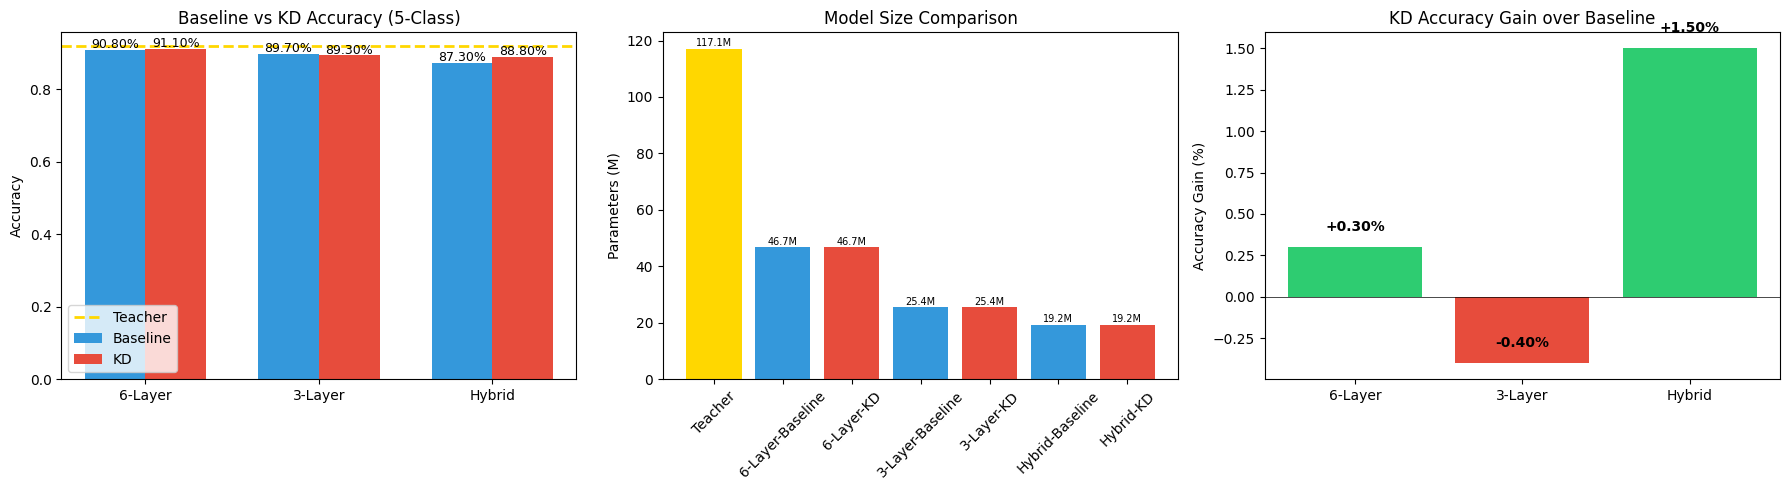
\includegraphics[width=\columnwidth]{multiclass_1.png}
\caption{Multiclass (5-class) with augmentation. \textbf{Left:} Baseline vs.\ KD accuracy. \textbf{Center:} Model sizes. \textbf{Right:} KD accuracy gain over baseline.}
\label{fig:multiclass_aug}
\end{figure}

Fig.~\ref{fig:dark_knowledge} illustrates why soft labels carry richer signal than hard labels. At temperature $T\!=\!5.0$, the teacher's output distribution reveals inter-class similarities---e.g., Splice~A samples show nonzero probability for other splice classes---providing the student with ``dark knowledge'' that hard one-hot labels cannot convey~\cite{hinton2015distilling}.

\begin{figure}[t]
\centering
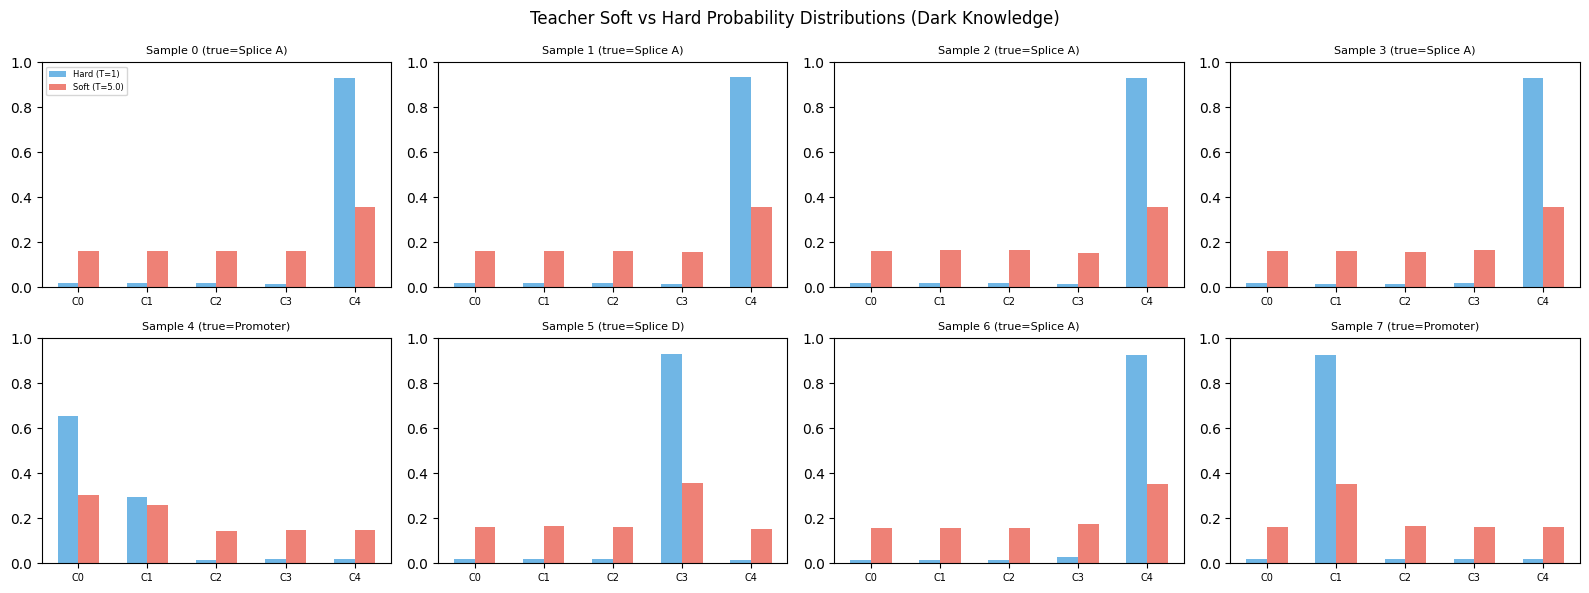
\includegraphics[width=\columnwidth]{multiclass_2.png}
\caption{Teacher soft vs.\ hard probability distributions on 5-class samples. Hard labels ($T\!=\!1$, blue) are near one-hot; soft labels ($T\!=\!5$, red) reveal inter-class structure that guides the student.}
\label{fig:dark_knowledge}
\end{figure}

\begin{table}[t]
\centering
\caption{5-class multiclass results ($\alpha\!=\!0.5$, $T\!=\!3.0$). KD $\Delta$ = accuracy change from KD vs.\ baseline.}
\label{tab:multiclass_aug}
\setlength{\tabcolsep}{3.5pt}
\begin{tabular}{llcccc}
\toprule
\textbf{Setting} & \textbf{Model} & \textbf{Acc.} & \textbf{F1} & \textbf{Params} & \textbf{KD $\Delta$} \\
\midrule
\multirow{5}{*}{\rotatebox[origin=c]{90}{\scriptsize No Aug}}
& Teacher        & 96.60 & .966 & 117.1M & --- \\
& 6L Baseline    & 75.10 & .741 & 46.7M  & --- \\
& 6L + KD        & 73.70 & .724 & 46.7M  & \textcolor{red}{$-$1.4} \\
& Hybrid Base    & 83.00 & .829 & 19.2M  & --- \\
& Hybrid + KD    & 86.80 & .868 & 19.2M  & \textcolor{green!60!black}{$+$3.8} \\
\midrule
\multirow{7}{*}{\rotatebox[origin=c]{90}{\scriptsize With Aug}}
& Teacher        & 91.80 & .918 & 117.1M & --- \\
& 6L Baseline    & 90.80 & .908 & 46.7M  & --- \\
& 6L + KD        & 91.10 & .911 & 46.7M  & \textcolor{green!60!black}{$+$0.3} \\
& 3L Baseline    & 89.70 & .897 & 25.4M  & --- \\
& 3L + KD        & 89.30 & .893 & 25.4M  & \textcolor{red}{$-$0.4} \\
& Hybrid Base    & 87.30 & .873 & 19.2M  & --- \\
& Hybrid + KD    & \textbf{88.80} & .887 & 19.2M  & \textcolor{green!60!black}{$+$1.5} \\
\bottomrule
\end{tabular}
\end{table}

\subsection{Cross-Species Generalization}

We evaluate models trained on \emph{human} promoters on two unseen species groups (Table~\ref{tab:crossspecies}). No retraining is performed.

\begin{table}[t]
\centering
\caption{Cross-species generalization. Drop = Human Acc $-$ Cross-species Acc (lower is better).}
\label{tab:crossspecies}
\setlength{\tabcolsep}{3.5pt}
\begin{tabular}{lccccc}
\toprule
\textbf{Model} & \textbf{Human} & \textbf{Mouse} & \textbf{Plant} & \multicolumn{2}{c}{\textbf{Drop}} \\
& Acc & Acc & Acc & Mouse & Plant \\
\midrule
Teacher (DNABERT-2)   & 96.71 & 79.66 & 48.22 & 17.04 & 48.48 \\
Hybrid (init.)    & 93.31 & \textbf{82.61} & 47.48 & \textbf{10.70} & 45.83 \\
4L-Pure-Trans. (KD) & 93.01 & 82.24 & 46.20 & 10.76 & 46.80 \\
\bottomrule
\end{tabular}
\end{table}

\textbf{Surprising result}: Both distilled students \emph{outperform} the teacher on mouse promoters despite being $3.6$--$4.5\times$ smaller. The Hybrid achieves 82.61\% and the 4L-Pure-Transformer achieves 82.24\%, compared to the teacher's 79.66\%. Their accuracy drops from human to mouse ($\sim$10.7\%) are far smaller than the teacher's 17.04\%, indicating substantially better cross-species transfer within mammals.

Remarkably, the pure transformer---trained entirely from scratch---nearly matches the DNABERT-2-initialized Hybrid on mouse data (82.24\% vs.\ 82.61\%), confirming that KD transfers generalizable features regardless of student initialization.

On plant promoters (different kingdom), all models perform near chance ($\sim$46--48\%), which is expected given the vast evolutionary distance and divergent regulatory grammar between mammals and plants.

\begin{figure}[t]
\centering
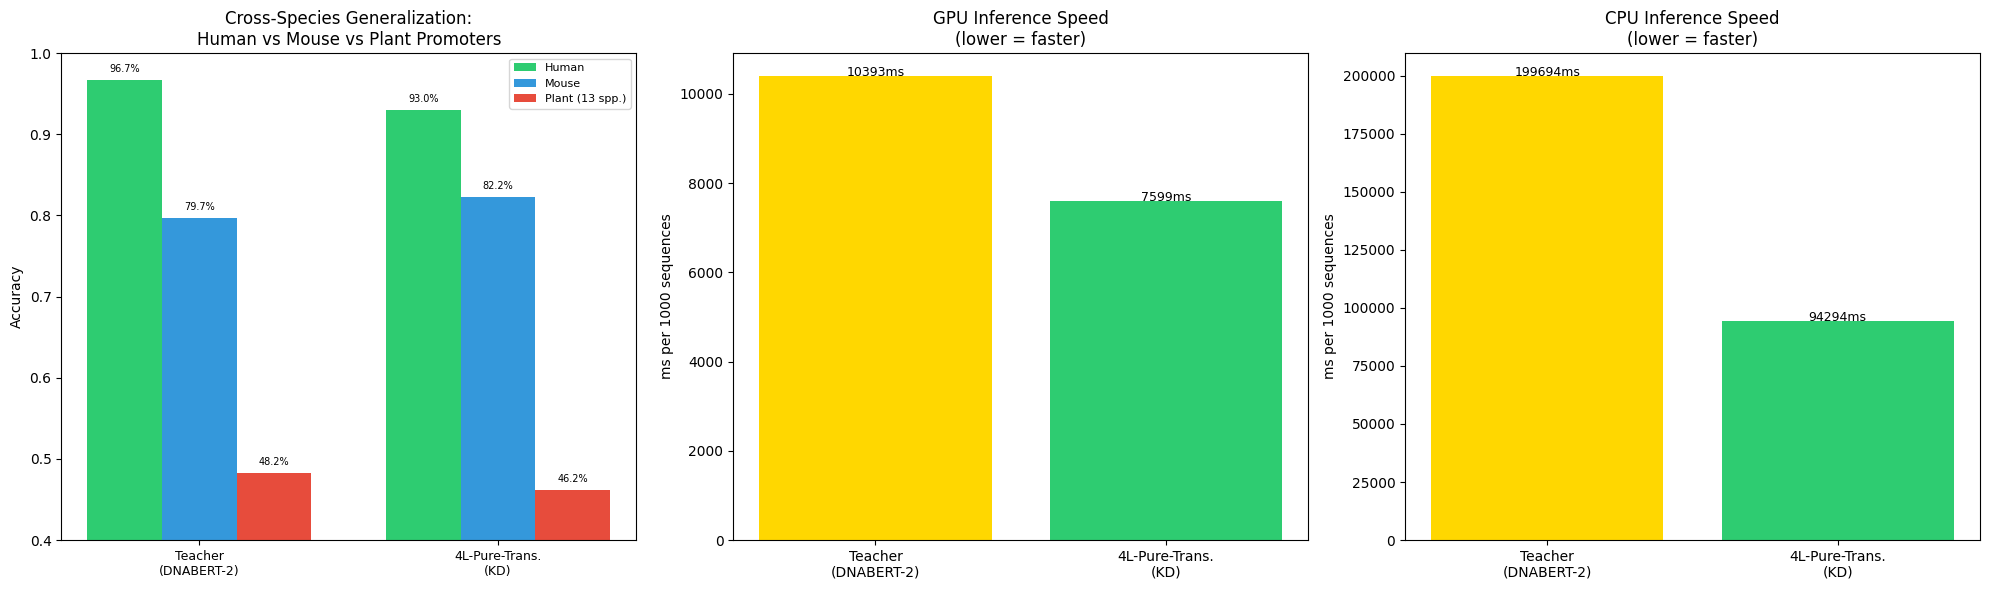
\includegraphics[width=\columnwidth]{pure_arch_gen_speed.png}
\caption{4L-Pure-Transformer (KD) evaluation. \textbf{Left:} Cross-species accuracy (teacher vs.\ student). \textbf{Center:} GPU speed. \textbf{Right:} CPU speed.}
\label{fig:gen_speed}
\end{figure}

\subsection{Inference Speed Benchmark}

Table~\ref{tab:speed} reports inference latency measured on 1,000 sequences with 3 warmup passes and \texttt{torch.cuda.synchronize()} for GPU timing.

\begin{table}[t]
\centering
\caption{Inference speed (ms per 1,000 sequences, batch size 16).}
\label{tab:speed}
\setlength{\tabcolsep}{3.5pt}
\begin{tabular}{lrrrr}
\toprule
\textbf{Model} & \textbf{GPU ms} & \textbf{CPU ms} & \textbf{GPU $\uparrow$} & \textbf{CPU $\uparrow$} \\
\midrule
Teacher (DNABERT-2)  & 10,059 & 197,053 & $1.00\times$ & $1.00\times$ \\
Hybrid (init.)   & 5,890  & 72,911  & $1.71\times$ & $\mathbf{2.70\times}$ \\
4L-Pure-Trans.   & 7,599  & 94,295  & $1.37\times$ & $2.12\times$ \\
\bottomrule
\end{tabular}
\end{table}

The Hybrid student is $1.71\times$ faster on GPU and $2.70\times$ faster on CPU, while the 4L-Pure-Transformer achieves $1.37\times$ GPU and $2.12\times$ CPU speedups. The Hybrid's larger CPU speedup reflects its CNN head's efficiency---convolutions are well-optimized on CPUs. The pure transformer, despite having the same 32.5\,M parameters as the 4-Layer Standard, is faster than the teacher due to its shallower depth (4 vs.\ 12 layers).

% ============================================================
\section{Discussion}
\label{sec:discussion}

\subsection{Why KD Helps the Hybrid but Hurts the 6-Layer}

Without augmentation, KD degrades the 6-Layer student by 1.4\% while boosting the Hybrid by 3.8\%. We identify three factors:

\textbf{(1) Teacher overconfidence.}\quad
On the small 13.6K multiclass dataset, the teacher's training loss drops to 0.028, indicating memorization. Average soft-label entropy is only 1.515\,bits (vs.\ $\log_2 5 = 2.322$ max), meaning soft labels are near-one-hot and add noise rather than useful signal~\cite{hinton2015distilling, li2023curriculum}.

\textbf{(2) Capacity gap.}\quad
The teacher (117\,M) is only $2.5\times$ larger than the 6-Layer student (46.7\,M) but $6.1\times$ larger than the Hybrid (19.2\,M). Counterintuitively, the \emph{smaller} gap hurts more: the 6-Layer has enough capacity to overfit to noisy soft labels, while the Hybrid's limited capacity acts as implicit regularization, selectively absorbing only the most useful dark knowledge~\cite{mirzadeh2020improved}.

\textbf{(3) Inductive bias.}\quad
The Hybrid's CNN head with kernel size 9 provides a strong structural prior for DNA motifs (TATA box $\sim$10\,bp, CAAT box $\sim$8\,bp). This constrains the student to learn biologically relevant features, making it more robust to noisy teacher signals.

\subsection{Data Augmentation as Teacher Regularization}

With augmentation, teacher accuracy drops from 96.6\% to 91.8\%, and KD becomes beneficial even for the 6-Layer student ($+0.3\%$). Augmentation prevents teacher overfitting, producing softer, more informative distributions. This aligns with Tang et al.~\cite{tang2020understanding}, who showed that teacher calibration is a key determinant of KD success. We recommend \emph{always augmenting before distillation} on datasets with $<$20K training samples.

\subsection{Cross-Species Generalization}

Both distilled students outperform the teacher on mouse promoters (82.61\% and 82.24\% vs.\ 79.66\%) despite lower human accuracy, suggesting that distillation acts as a \emph{regularizer against species-specific overfitting}. The teacher memorizes human-specific promoter patterns, while the students' constrained capacity forces them to learn more generalizable motifs shared across mammals.

That the pure transformer---with no pretrained weights---nearly matches the DNABERT-2-initialized Hybrid on mouse data is particularly noteworthy: it implies the generalization benefit comes from the distillation process itself, not from the teacher's pretrained representations being inherited through weight initialization.

The near-random performance on plant promoters for all models confirms that mammalian promoter features do not transfer across kingdoms, consistent with the fundamental differences in plant vs.\ animal transcriptional regulation.

\subsection{Pure Architectures: KD Without Pretraining}

The consistent $\sim$1\% KD gain across all three pure architectures (Table~\ref{tab:pure_arch}) demonstrates that KD is effective even without pretrained initialization, though the absolute improvement is smaller than the $\sim$3.8\% gains seen for pretrained Hybrids on multiclass tasks. The 4L-Pure-Transformer's 93.01\% accuracy is only 0.30 points below the DNABERT-2-initialized Hybrid (93.31\%), suggesting that for binary promoter classification, the teacher's soft-label guidance can largely compensate for the lack of pretrained weights.

The 4L-Pure-CNN's poor accuracy (84.83\%) confirms that self-attention is essential for capturing long-range dependencies in promoter sequences, while the Hybrid-Pure-3T1C (92.85\%) benefits from both local (CNN) and global (transformer) pattern detection.

\subsection{Practical Deployment Considerations}

The Hybrid student's $2.7\times$ CPU speedup and 105\,MB model size make it deployable on standard laptops---processing 1,000 sequences in $\sim$73 seconds on CPU vs.\ $\sim$197 seconds for the teacher. For laboratories without GPU access, this represents a meaningful practical improvement.

% ============================================================
\section{Conclusion}
\label{sec:conclusion}

We presented a systematic study of knowledge distillation for compressing DNABERT-2 for DNA promoter classification. Our key findings are:

\begin{enumerate}
    \item A \textbf{Hybrid CNN-Transformer} student (26.3\,M params, $4.5\times$ compression) achieves 93.31\% accuracy---96.5\% of the teacher---with $2.7\times$ CPU speedup.
    \item A \textbf{4L-Pure-Transformer} trained from scratch with KD achieves 93.01\%, demonstrating that KD effectively transfers knowledge without pretrained initialization.
    \item Both distilled students \textbf{outperform the teacher on mouse promoters} ($>$82\% vs.\ 79.66\%), showing that KD improves cross-species generalization.
    \item \textbf{Lower $\alpha$} ($\alpha\!=\!0.3$) and \textbf{moderate temperature} ($T\!=\!3.0$) are optimal for the Hybrid architecture.
    \item \textbf{Data augmentation is essential} for KD on small multiclass datasets, regularizing overconfident teachers to produce informative soft labels.
\end{enumerate}

Future work includes adaptive per-sample temperatures, motif-aware intermediate distillation, and combining KD with INT8 quantization for further compression.

% ============================================================
\bibliographystyle{IEEEtranN}
\begin{thebibliography}{12}

\bibitem{hinton2015distilling}
G.~Hinton, O.~Vinyals, and J.~Dean,
``Distilling the knowledge in a neural network,''
\emph{arXiv:1503.02531}, 2015.

\bibitem{ji2021dnabert}
Y.~Ji, Z.~Zhou, H.~Liu, and R.~V.~Davuluri,
``{DNABERT}: pre-trained bidirectional encoder representations from transformers model for {DNA}-language in genome,''
\emph{Bioinformatics}, vol.~37, no.~15, pp.~2112--2120, 2021.

\bibitem{zhou2023dnabert2}
Z.~Zhou, Y.~Ji, W.~Li, P.~Dutta, R.~Davuluri, and H.~Liu,
``{DNABERT-2}: Efficient foundation model and benchmark for multi-species genome,''
\emph{arXiv:2306.15006}, 2023.

\bibitem{dallatorre2023nucleotide}
H.~Dalla-Torre, L.~Gonzalez, J.~Mendoza-Revilla, \emph{et~al.},
``The {Nucleotide Transformer}: Building and evaluating robust foundation models for human genomics,''
\emph{bioRxiv}, 2023.

\bibitem{sanh2019distilbert}
V.~Sanh, L.~Debut, J.~Chaumond, and T.~Wolf,
``{DistilBERT}, a distilled version of {BERT}: smaller, faster, cheaper and lighter,''
\emph{arXiv:1910.01108}, 2019.

\bibitem{jiao2020tinybert}
X.~Jiao, Y.~Yin, L.~Shang, X.~Jiang, X.~Chen, L.~Li, F.~Wang, and Q.~Liu,
``{TinyBERT}: Distilling {BERT} for natural language understanding,''
in \emph{Findings of EMNLP}, pp.~4163--4174, 2020.

\bibitem{mirzadeh2020improved}
S.~I.~Mirzadeh, M.~Farajtabar, A.~Li, N.~Levine, A.~Matsukawa, and H.~Ghasemzadeh,
``Improved knowledge distillation via teacher assistant,''
in \emph{AAAI}, pp.~5191--5198, 2020.

\bibitem{li2023curriculum}
C.~Li, H.~Yang, J.~Zhang, \emph{et~al.},
``Curriculum temperature for knowledge distillation,''
in \emph{AAAI}, 2023.

\bibitem{tang2020understanding}
J.~Tang, R.~Shivanna, Z.~Zhao, D.~Lin, A.~Singh, E.~H.~Chi, and S.~Jain,
``Understanding and improving knowledge distillation,''
\emph{arXiv:2002.03532}, 2020.

\bibitem{oubounyt2019deepromoter}
M.~Oubounyt, Z.~Louadi, H.~Tayara, and K.~T.~Chong,
``{DeePromoter}: Robust promoter predictor using deep learning,''
\emph{Frontiers in Genetics}, vol.~10, p.~286, 2019.

\bibitem{zhangtaolab2024plant}
{Zhang Lab},
``Plant multi-species core promoters,''
\emph{Hugging Face Datasets}, 2024.
\url{https://huggingface.co/datasets/zhangtaolab/plant-multi-species-core-promoters}.

\bibitem{muller2019does}
R.~M{\"u}ller, S.~Kornblith, and G.~Hinton,
``When does label smoothing help?''
in \emph{NeurIPS}, pp.~4694--4703, 2019.

\bibitem{instadeep2023dataset}
{InstaDeep},
``Nucleotide transformer downstream tasks,''
\emph{Hugging Face Datasets}, 2023.
\url{https://huggingface.co/datasets/InstaDeepAI/nucleotide_transformer_downstream_tasks}.

\end{thebibliography}

\balance
\end{document}
